\documentclass[border=5pt]{standalone}

\usepackage{amsfonts,amssymb,amsmath}
\usepackage{tikz}
\usetikzlibrary{matrix}

\newcommand{\BO}{\mathrm{BO}}
\newcommand{\BSO}{\mathrm{BSO}}
\newcommand{\BSpin}{\mathrm{BSpin}}

\newcommand{\zz}{\ensuremath\mathbb{Z}_2}
\newcommand{\Z}{\ensuremath\mathbb{Z}}

\tikzset{ 
table/.style={
  matrix of nodes,
  row sep=-\pgflinewidth,
  column sep=-\pgflinewidth,
  nodes={rectangle,text width=3em,align=center},
  text depth=1.25ex,
  text height=2.5ex,
  nodes in empty cells
},
row 1/.style={nodes={fill=gray!20,text depth=0.4ex,text height=2ex}},
column 1/.style={nodes={rectangle, text width=8em,align=center}}
}

\begin{document}
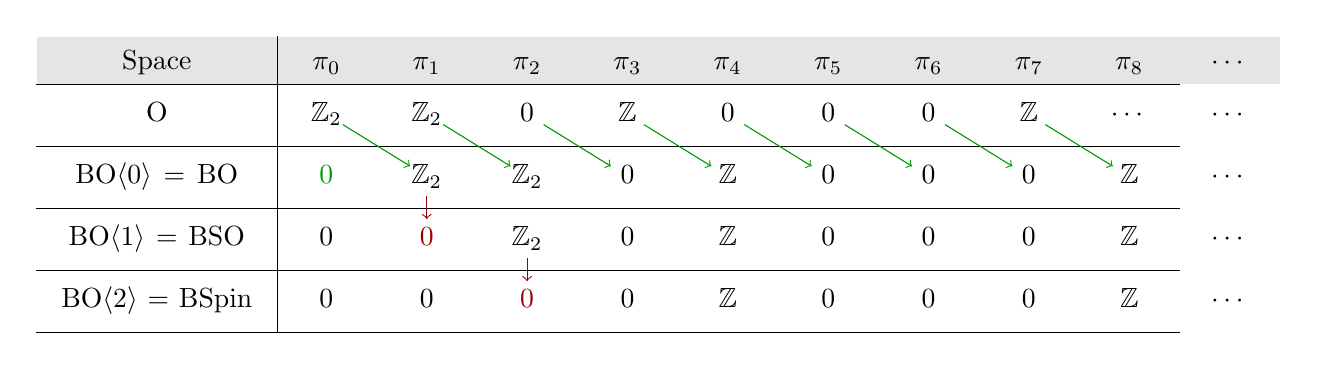
\begin{tikzpicture}
\matrix (mat) [table] {
    Space & $\pi_0$ & $\pi_1$ & $\pi_2$ & $\pi_3$ & $\pi_4$ & $\pi_5$ & $\pi_6$ & $\pi_7$ & $\pi_8$ & $\cdots$\\
    $\mathrm{O}$ & $\zz$ & $\zz$ & $0$ & $\Z$ & $0$ & $0$ & $0$ & $\Z$ & $\cdots$ & $\cdots$  \\
    $\BO\langle 0\rangle = \BO$ & {\color{green!60!black} $0$} & $\zz$ & $\zz$ & $0$ & $\Z$ & $0$ & $0$ & $0$ & $\Z$ & $\cdots$ \\
    $\BO\langle 1\rangle = \BSO$ & $0$ & {\color{red!60!black} $0$} & $\zz$ & $0$ & $\Z$ & $0$ & $0$ & $0$ & $\Z$ & $\cdots$ \\
    $\BO\langle 2\rangle = \BSpin$ & $0$ & $0$ & {\color{red!60!black} $0$} & $0$ & $\Z$ & $0$ & $0$ & $0$ & $\Z$ & $\cdots$ \\
};
% the matrix rules
\foreach \x in {1,...,5}
{
  \draw
    ([xshift=-.5\pgflinewidth]mat-\x-1.south west) --
    ([xshift=-.5\pgflinewidth]mat-\x-10.south east);
  }
\draw
    ([yshift=.5\pgflinewidth]mat-1-1.north east) --
    ([yshift=.5\pgflinewidth]mat-5-1.south east);
% the arrows
\begin{scope}[shorten >=7pt,shorten <=7pt]
\foreach \x in {2,...,9}
{
    \pgfmathtruncatemacro{\y}{\x + 1};
    \draw[->, green!60!black] (mat-2-\x.center) -- (mat-3-\y.center);
}
    \draw[->, red!60!black] (mat-3-3.center) -- (mat-4-3.center);
    \draw[->, red!60!black] (mat-4-4.center) -- (mat-5-4.center);
\end{scope}
\end{tikzpicture}
\end{document}
